\begin{equation}
    \begin{gathered}
        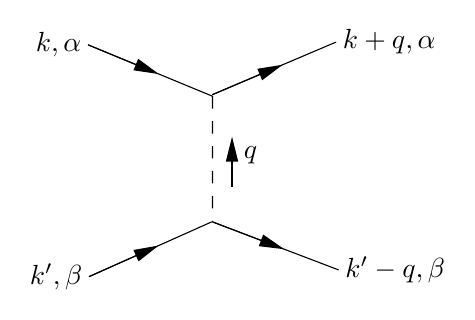
\begin{tikzpicture}[x=0.75pt,y=0.75pt,yscale=-1,xscale=1]
            %uncomment if require: \path (0,300); %set diagram left start at 0, and has height of 300
            %Straight Lines [id:da6810974252980533] 
            \draw    (120.17,187.49) -- (151.95,173.3) ;
            \draw [shift={(153.77,172.48)}, rotate = 515.9300000000001] [fill={rgb, 255:red, 0; green, 0; blue, 0 }  ][line width=0.08]  [draw opacity=0] (12,-3) -- (0,0) -- (12,3) -- cycle    ;
            %Straight Lines [id:da40733827497945274] 
            \draw    (120.17,187.49) -- (179.26,161.1) ;
            
            %Straight Lines [id:da4271611228799128] 
            \draw    (179.7,161.1) -- (212.38,173.55) ;
            \draw [shift={(214.25,174.26)}, rotate = 200.85] [fill={rgb, 255:red, 0; green, 0; blue, 0 }  ][line width=0.08]  [draw opacity=0] (12,-3) -- (0,0) -- (12,3) -- cycle    ;
            %Straight Lines [id:da753337349268864] 
            \draw    (179.7,161.1) -- (240.46,184.24) ;
            
            %Straight Lines [id:da09481485705124859] 
            \draw    (119.72,75.78) -- (151.97,89.1) ;
            \draw [shift={(153.82,89.87)}, rotate = 202.44] [fill={rgb, 255:red, 0; green, 0; blue, 0 }  ][line width=0.08]  [draw opacity=0] (12,-3) -- (0,0) -- (12,3) -- cycle    ;
            %Straight Lines [id:da7578837470001811] 
            \draw    (119.72,75.78) -- (179.69,100.55) ;
            
            %Straight Lines [id:da7058048331027083] 
            \draw    (179.57,99.82) -- (211.65,86.18) ;
            \draw [shift={(213.49,85.39)}, rotate = 516.96] [fill={rgb, 255:red, 0; green, 0; blue, 0 }  ][line width=0.08]  [draw opacity=0] (12,-3) -- (0,0) -- (12,3) -- cycle    ;
            %Straight Lines [id:da4335041927311629] 
            \draw    (179.57,99.82) -- (239.22,74.45) ;
            
            %Straight Lines [id:da2943384130706994] 
            \draw    (189.09,144.08) -- (189.09,122.03) ;
            \draw [shift={(189.09,120.03)}, rotate = 450] [fill={rgb, 255:red, 0; green, 0; blue, 0 }  ][line width=0.08]  [draw opacity=0] (12,-3) -- (0,0) -- (12,3) -- cycle    ;
            %Straight Lines [id:da5722731848454237] 
            \draw  [dash pattern={on 4.5pt off 4.5pt}]  (179.69,100.55) -- (179.7,161.1) ;
            
            % Text Node
            \draw (117.72,75.78) node [anchor=east] [inner sep=0.75pt]    {$\boldsymbol{k} ,\alpha $};
            % Text Node
            \draw (241.22,74.45) node [anchor=west] [inner sep=0.75pt]    {$\boldsymbol{k} +\boldsymbol{q} ,\alpha $};
            % Text Node
            \draw (193.48,123.48) node [anchor=north west][inner sep=0.75pt]    {$\boldsymbol{q}$};
            % Text Node
            \draw (118.17,187.49) node [anchor=east] [inner sep=0.75pt]    {$\boldsymbol{k} ',\beta $};
            % Text Node
            \draw (242.46,184.24) node [anchor=west] [inner sep=0.75pt]    {$\boldsymbol{k} '-\boldsymbol{q} ,\beta $};
            \end{tikzpicture}
    \end{gathered} = - \frac{1}{\beta} \sum_{\omega_n} \int \frac{\dd[3]{\vb*{q}}}{(2\pi)^3} V_{\vb*{q}}  ,
\end{equation}